%----------------------------------------------%
%---------------- INTRODUCCIÓN ----------------%
%----------------------------------------------%

\framecard{COMUNIDAD DE KICAD}

\begin{frame}{Comunidad de Kicad}
	\begin{center}
	\begin{minipage}{0.7\textwidth}
	\begin{fullpageitemize}
		\item[\faCode] Launchpad: \href{https://launchpad.net/kicad}{launchpad.net/kicad} \\
		\pause
		\item[\faEnvelope] Lista de correo: \href{http://lists.launchpad.net/kicad-developers}{kicad-developers} \\
		\pause
		\item[\faHashtag] IRC: \#kicad \\
		\pause
		\item[\faUsers] Foro: \href{https://forum.kicad.info/}{forum.kicad.info} \\
		\pause
		\item[\faGithub] Github: \href{https://github.com/kicad/}{github.com/kicad/}
	\end{fullpageitemize}
	\end{minipage}
	\end{center}
\end{frame} 

\framecard{CÓMO COMPILAR}

\begin{frame}{Compilación}
	\inputminted[fontsize=\large]{bash}{code/get-kicad.sh}
\end{frame}

%\begin{frame}
	%\inputminted[firstline=200, lastline=240, fontsize=\small, linenos]{python}{code/python/start.py}
%\end{frame}

\framecard{ESTRUCTURA DEL CÓDIGO}

\begin{frame}
	\centering
	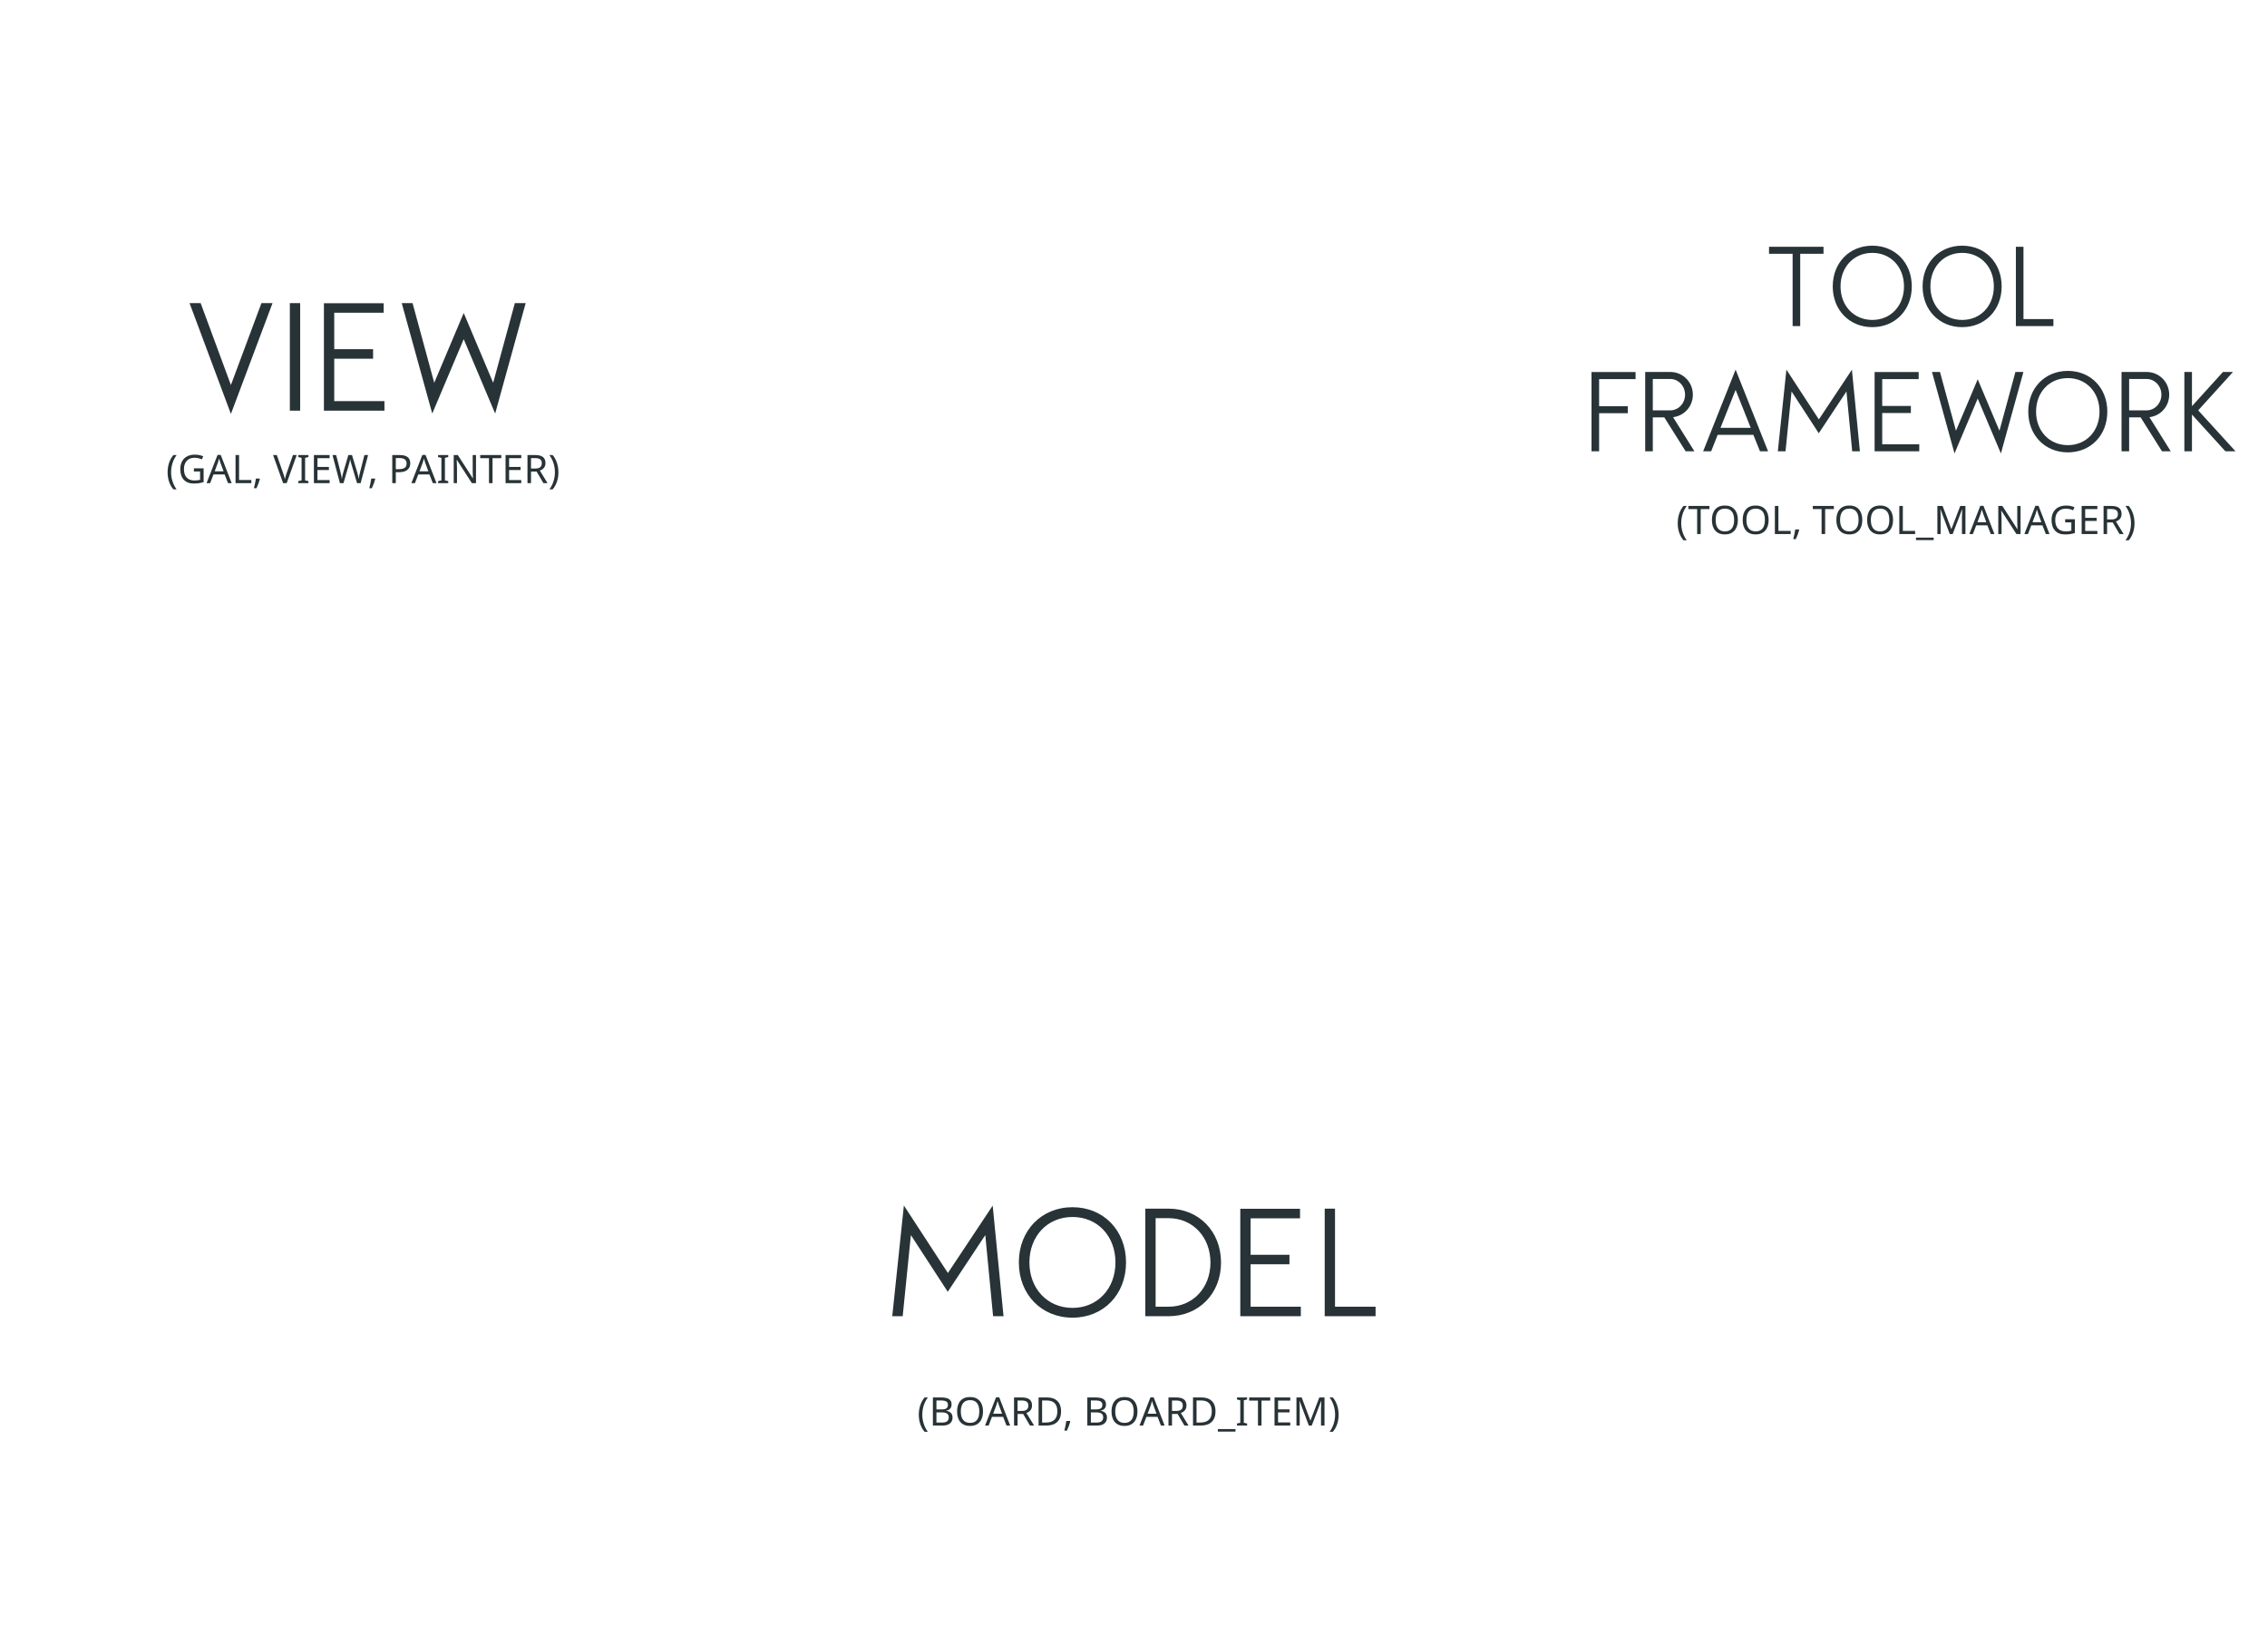
\includegraphics[width=0.8\textwidth]{gfx/tool_framework.png}
\end{frame}


\framecard{NUEVAS HERRAMIENTAS}

\begin{frame}{Nuevas herramientas}{Esqueleto}
	\begin{center}
		\begin{minipage}{0.9\textwidth}
			\inputminted{cpp}{code/cpp/tool_skeleton.cpp}
		\end{minipage}
	\end{center}
\end{frame}

\begin{frame}{Nuevas herramientas}{Constructor y destructor}
	\begin{center}
	\begin{minipage}{0.7\textwidth}
		\inputminted{cpp}{code/cpp/tool_constructor.cpp}
	\end{minipage}
	\end{center}
\end{frame}

\begin{frame}{Nuevas herramientas}{Reset}
\begin{center}
\begin{minipage}{0.7\textwidth}
	\inputminted{cpp}{code/cpp/tool_reset.cpp}
\end{minipage}
\end{center}
\end{frame}

\begin{frame}{Nuevas herramientas}{Inicialización}
\begin{center}
\begin{minipage}{0.7\textwidth}
	\inputminted{cpp}{code/cpp/tool_init.cpp}
\end{minipage}
\end{center}
\end{frame}

\begin{frame}{Nuevas herramientas}{Eventos estáticos}
\begin{center}
\begin{minipage}{0.85\textwidth}
	\inputminted{cpp}{code/cpp/tool_transitions.cpp}
\end{minipage}
\end{center}
\end{frame}

\begin{frame}{Nuevas herramientas}{Eventos interactivos}
\begin{center}
\begin{minipage}{0.8\textwidth}
	\inputminted{cpp}{code/cpp/tool_transitions_interactive.cpp}
\end{minipage}
\end{center}
\end{frame}

\begin{frame}{Nuevas herramientas}{¿Cómo registrar la nueva herramienta?}
	\begin{center}
	\begin{minipage}{0.8\textwidth}
		\begin{itemize}
			\pause
			\item[\faCode] Añadir la cabecera a \mintinline{shell}{pcbnew/CMakeLists.txt}
			\pause
			\item[\faCode] Registrar la nueva herramienta en \mintinline{shell}{pcbnew/tools/tools_common.cpp}
			\pause
		\end{itemize}
	\end{minipage}
	\end{center}

	\begin{center}
		\begin{minipage}{0.95\textwidth}
			\inputminted[fontsize=\small]{cpp}{code/cpp/register_tool.cpp}
		\end{minipage}
	\end{center}
\end{frame}

\framecard{\href{http://docs.kicad-pcb.org/doxygen/classEDA__ITEM.html}{CLASES DEL MODELO}}

\framecard{\href{http://docs.kicad-pcb.org/doxygen/classPCB__BASE__FRAME.html}{CLASES DE LA VISTA}}

\framecard{MAGIA NEGRA}

\begin{frame}
	\begin{center}
	\begin{minipage}{0.7\textwidth}
		\inputminted[fontsize=\large]{cpp}{code/cpp/commit.cpp}
	\end{minipage}
\end{center}
\end{frame}

\framecard{INTERACCIÓN}

\begin{frame}{Interacción con otras herramientas}
\begin{center}
	\begin{minipage}{0.7\textwidth}
		\only<1>{\inputminted[firstline=1, lastline=7, fontsize=\large]{cpp}{code/cpp/tool_action.cpp}}
		\only<2>{\inputminted[firstline=9, lastline=12, fontsize=\large]{cpp}{code/cpp/tool_action.cpp}}
		\only<3>{\inputminted[firstline=14, lastline=17, fontsize=\large]{cpp}{code/cpp/tool_action.cpp}}
	\end{minipage}
\end{center}
\end{frame}

\framecard{ENVIAR CONTRIBUCIONES}

\begin{frame}{¿Cómo enviar una contribución?}
		\begin{center}
		\begin{minipage}{0.8\textwidth}
			\begin{fullpageitemize}
				\item[\faCode] \mintinline{shell}{git clone https://git.launchpad.net/kicad} \\
				\pause
				\item[\faCode] \mintinline{shell}{Code all day long} \\
				\pause
				\item[\faCode] \mintinline{shell}{git add magic_code.cpp} \\
				\pause
				\item[\faCode] \mintinline{shell}{git commit -m "Black magic"} \\
				\pause
				\item[\faCode] \mintinline{shell}{git format-patch --attach origin/master}
			\end{fullpageitemize}
		\end{minipage}
	\end{center}	
\end{frame}

\framecard{C++ MOLA}

\framecard{PERO PYTHON MOLA MÁS}

\begin{frame}{Python}{Primeros pasos}
	  \begin{center}
		\begin{minipage}{0.8\textwidth}
			\inputminted[fontsize=\Large]{python}{code/python/start.py}
		\end{minipage}
	\end{center}
\end{frame}

\begin{frame}{Python}{Primeros pasos}
	\inputminted[fontsize=\large]{python}{code/python/nets.py}
\end{frame}

\begin{frame}{Python}{Primeros pasos}
\begin{center}
	\begin{minipage}{0.9\textwidth}
		\inputminted[fontsize=\large]{python}{code/python/nets2.py}
	\end{minipage}
\end{center}
\end{frame}

\framecard{ALGO MÁS AVANZADO}

\begin{frame}{Interacción con otras herramientas}
\begin{center}
	\begin{minipage}{0.8\textwidth}
		\only<1>{\inputminted[firstline=1, lastline=7, fontsize=\large]{cpp}{code/python/add_track.py}}
		\only<2>{\inputminted[firstline=9, lastline=15, fontsize=\large]{cpp}{code/python/add_track.py}}
		\only<3>{\inputminted[firstline=17, lastline=24, fontsize=\large]{cpp}{code/python/add_track.py}}
		\only<4>{\inputminted[firstline=26, lastline=28, fontsize=\large]{cpp}{code/python/add_track.py}}
	\end{minipage}
\end{center}
\end{frame}

\begin{frame}{Referencias}
	\begin{center}
	\begin{minipage}{0.8\textwidth}
		El código de esta presentación se encuentra en \faGithub\href{https://github.com/agarciamontoro/contribuyendo-a-kicad}{agarciamontoro/contribuyendo-a-kicad} y está basada en: \\
	\end{minipage}
	\begin{minipage}{0.7\textwidth}
		\begin{fullpageitemize}
			\pause
			\item[\faComments] \href{https://fosdem.org/2017/schedule/event/kicad_source/attachments/slides/1696/export/events/attachments/kicad_source/slides/1696/kicad_source.pdf}{Charla de Orson en FOSDEM '17} \\
			\pause
			\item[\faWordpress] \href{https://kicad.mmccoo.com/}{Blog de mmccoo} \\
		\end{fullpageitemize}
	\end{minipage}
\end{center}
\end{frame}